\section{Zusätzliche Persona}

Um die Software im Folgenden in den Kategorien des Inklusive Designs testen zu können, wir zunächst eine weitere Persona erstellt.
Diese Persona verfügt über Eigenschaften, welche gewisse Barrierefreiheiten der Software voraussetzt.
Es wird nun zunächst die zusätzliche Persona, Lina Schneider, vorgestellt.
Daraufhin wird die Software mit Hilfe dieser und den Inklusive Design Support Cards \cite{ITToolkit} untersucht und an nötigen Stellen angepasst.

\autoref{fig:persona-lina} zeigt eine grafische Darstellung der Persona Lina Schneider.
Lina hat einen zweijährigen Sohn namens Jonas.
Nach der Elternzeit möchte sie nun wieder in ihren Job zurückkehren.
Ein Fahrradunfall, welcher einen gebrochenen Arm zu Folge hatte, erschwert ihr dies jedoch.
Da sie sich die Erziehung von Jonas mit ihrem Mann Moritz gut aufteilt, kann Lina trotz des Unfalls von Zuhause arbeiten.
Sie möchte trotz ihrer Einschränkungen an der Arbeit wie jede andere Person behandelt werden.

\begin{figure}[htp]
    \centering
    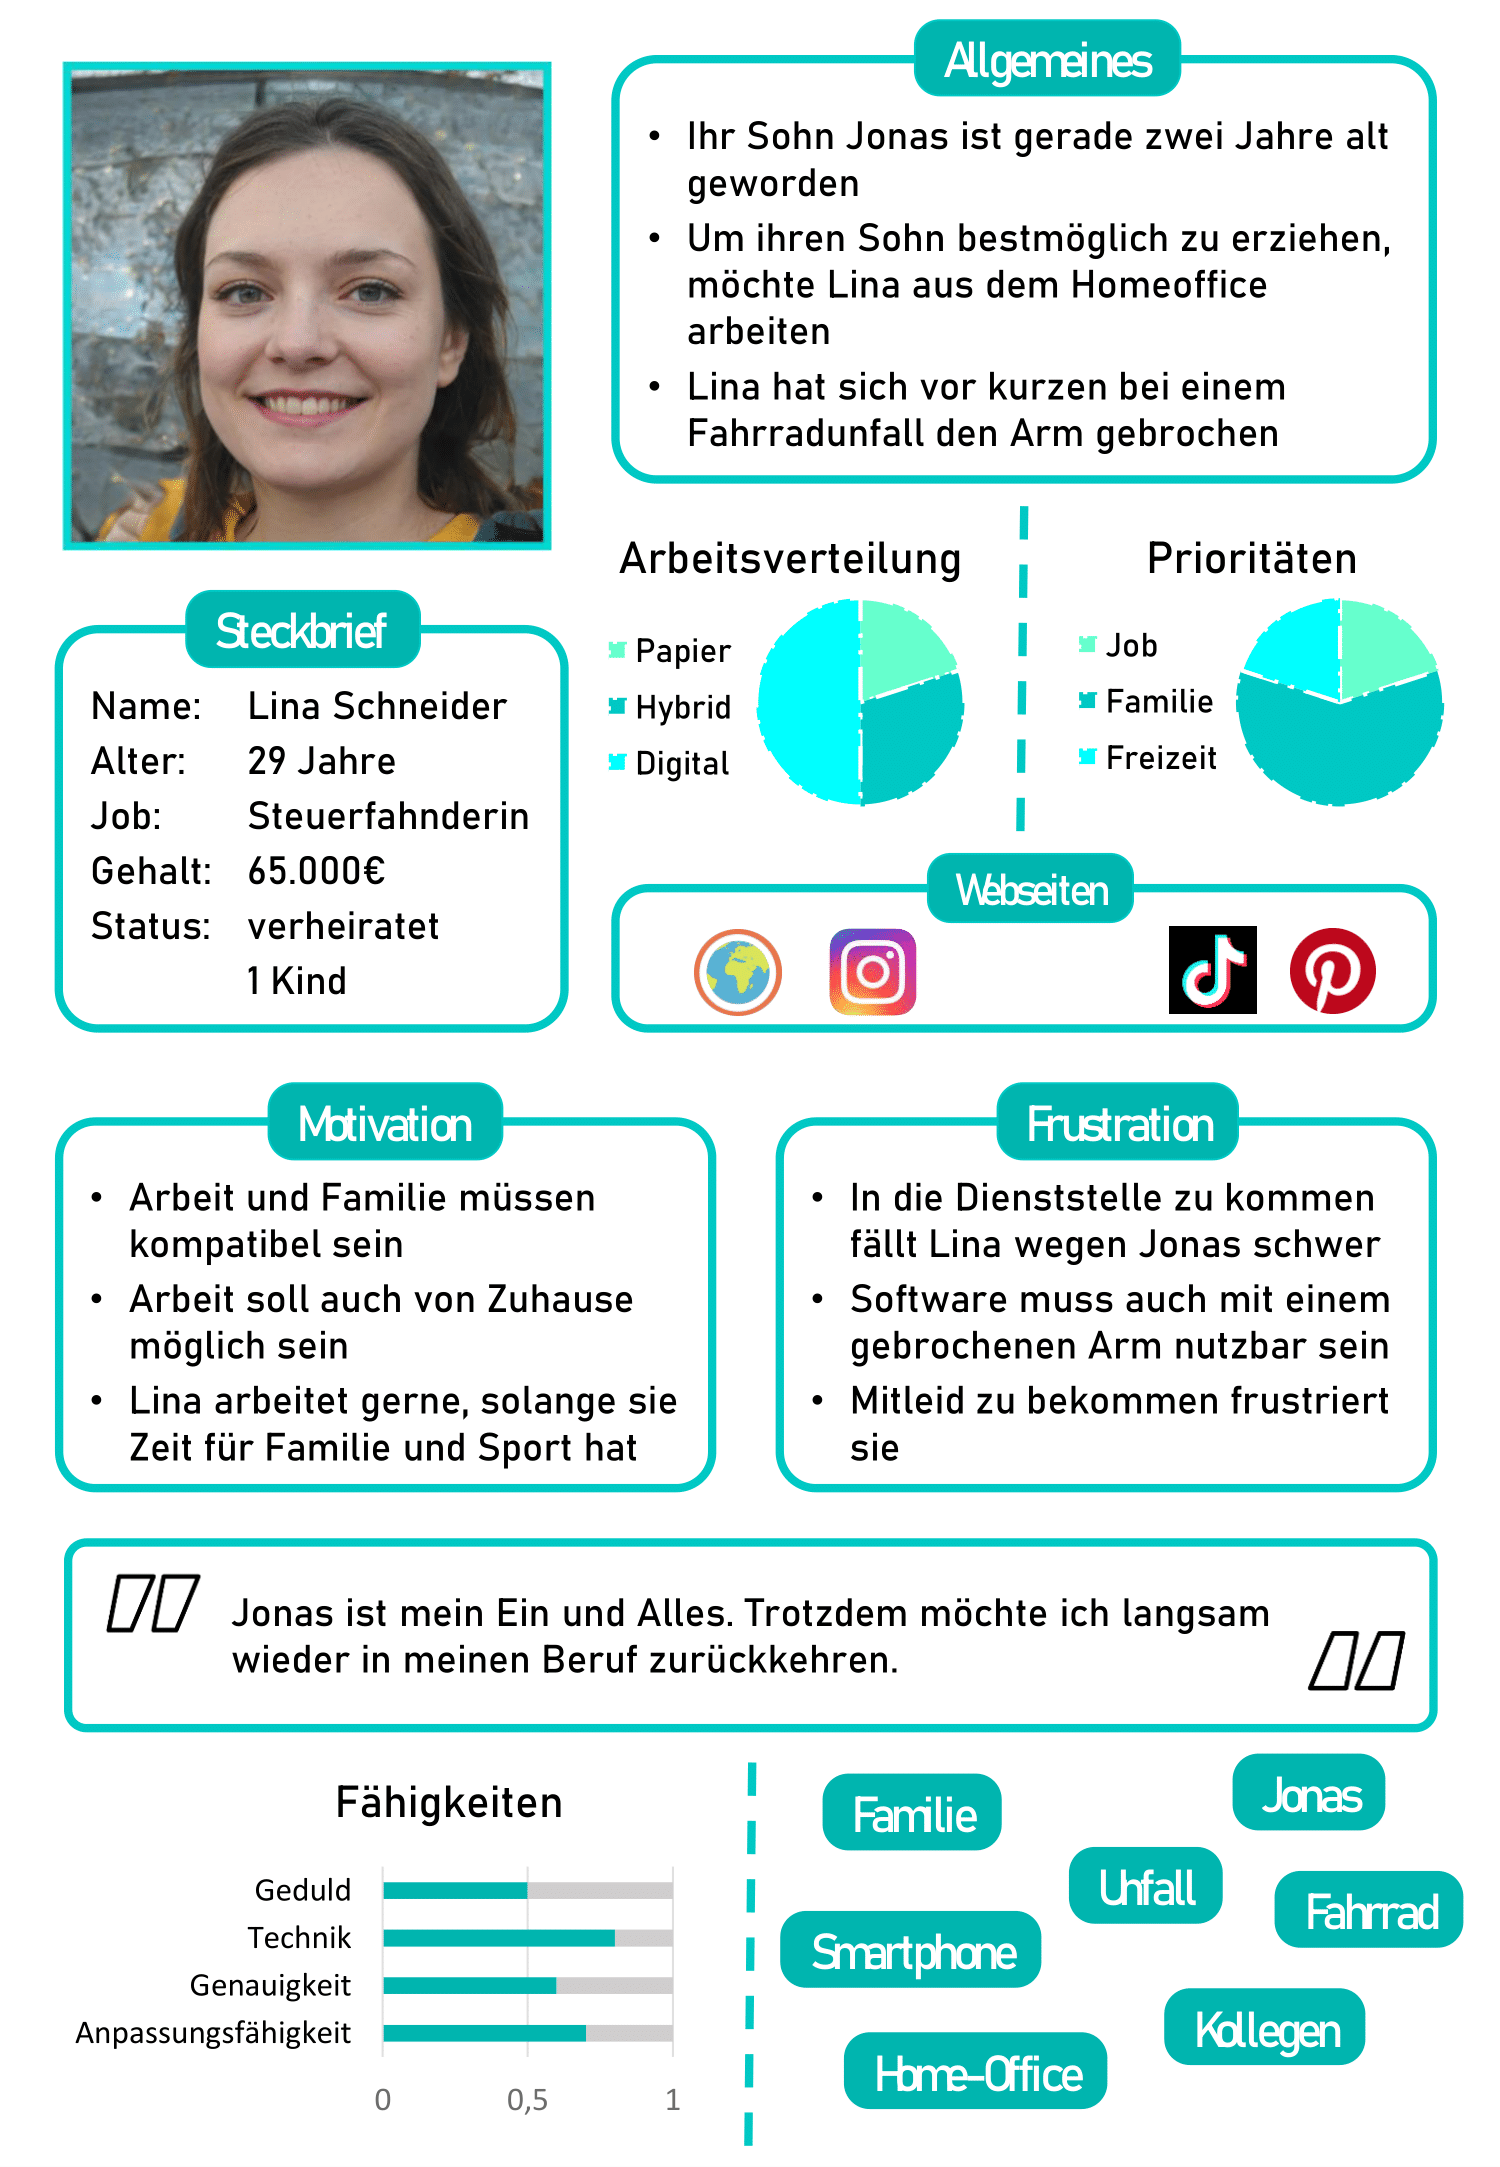
\includegraphics[width=\textwidth]{images/persona_2.png}
    \caption{Persona Lina Schneider}
    \label{fig:persona-lina}
\end{figure}